\documentclass[12pt, a4paper]{article}

\usepackage{graphicx}
\usepackage{xcolor}
\usepackage{float}
\usepackage{svg}
\usepackage[colorlinks=true, linkcolor=black, urlcolor=blue, citecolor=green]{hyperref}
\usepackage{enumitem}
\usepackage[italian]{babel}
\usepackage{lastpage}  % Pacchetto per ottenere il numero totale delle pagine
\usepackage{fancyhdr}  % Pacchetto per personalizzare l'intestazione e il piè di pagina
\usepackage[margin=1in]{geometry}
\usepackage{array}
\newcolumntype{C}[1]{>{\centering\arraybackslash}p{#1}}
\newcolumntype{L}[1]{>{\raggedright\arraybackslash}p{#1}}
\graphicspath{ {images/} {../shared/images/} }
\definecolor{unipd}{HTML}{B5121B}

\addto\captionsitalian{\renewcommand{\contentsname}{Indice}}


\pagestyle{fancy}% Imposta lo stile di pagina su "fancy"
\fancyhf{}% Cancella intestazioni e piè di pagina
\fancyfoot[C]{\thepage{} di \pageref{LastPage}} % Imposta il piè di pagina centrale come "numero pagina di totale pagine"
\renewcommand{\headrulewidth}{0pt} % Imposta la larghezza della linea di intestazione a 0 punti

% COMANDI PER CONTATORI
\newcounter{uccounter}
\newcommand{\uc}[2]{%
  \refstepcounter{uccounter}%
  \addcontentsline{toc}{subsubsection}{UC\arabic{uccounter}\ - #1}%
  \subsubsection*{\label{#2}\textbf{UC\arabic{uccounter}\ - #1}}%
}

\newcounter{subuccounter}[uccounter]
\newcommand{\subuc}[2]{%
  \refstepcounter{subuccounter}%
  \addcontentsline{toc}{subsubsection}{UC\arabic{uccounter}.\arabic{subuccounter}\ - #1}%
  \subsubsection*{\label{#2}\textbf{UC\arabic{uccounter}.\arabic{subuccounter}\ - #1}}%
}

\newcounter{subsubuccounter}[subuccounter]
\newcommand{\subsubuc}[2]{%
  \refstepcounter{subsubuccounter}%
  \addcontentsline{toc}{subsubsection}{UC\arabic{uccounter}.\arabic{subuccounter}.\arabic{subsubuccounter}\ - #1}%
  \subsubsection*{\label{#2}\textbf{UC\arabic{uccounter}.\arabic{subuccounter}.\arabic{subsubuccounter}\ - #1}}%
}

\newcounter{subsubsubuccounter}[subsubuccounter]
\newcommand{\subsubsubuc}[2]{%
  \refstepcounter{subsubsubuccounter}%
  \addcontentsline{toc}{subsubsection}{UC\arabic{uccounter}.\arabic{subuccounter}.\arabic{subsubuccounter}.\arabic{subsubsubuccounter}\ - #1}%
  \subsubsection*{\label{#2}\textbf{UC\arabic{uccounter}.\arabic{subuccounter}.\arabic{subsubuccounter}.\arabic{subsubsubuccounter}\ - #1}}%
}

% \newcommand{\data}{GG mese AAAA}
\newcommand{\titolo}{Analisi dei Requisiti}
% \newcommand{\responsabile}{Responsabile}
\newcommand{\verificatore}{
    & Davide Martinelli \\
    & Nome2 Cognome2 \\
    & Nome3 Cognome3 \\
}
\newcommand{\redattore}{
    & Nome1 Cognome1 \\
    & Nome2 Cognome2 \\
    & Nome3 Cognome3 \\
}
% \newcommand{\uso}{Interno/Esterno}
\newcommand{\destinatari }{
    & Tullio Vardanega \\
    & Riccardo Cardin \\
    & Vimar S.p.A. \\
    & Gruppo PEBKAC
}
\newcommand{\abstractcontent}{abstract ...}

\begin{document}

\begin{minipage}[]{0.3\textwidth}
\includesvg[width=\linewidth]{pebkac.svg} 
\end{minipage}
\hspace{0.05\textwidth}
\begin{minipage}[]{0.65\textwidth}
  {\Large \textbf{PEBKAC}} \\
  Gruppo: 11 \\
  Email: \href{mailto:pebkacswe@gmail.com}{pebkacswe@gmail.com} \\
  Docs: \href{https://pebkac-swe-group-11.github.io}{https://pebkac-swe-group-11.github.io} \\
  GitHub: \href{https://github.com/PEBKAC-SWE-Group-11}{https://github.com/PEBKAC-SWE-Group-11} \\
  
\end{minipage}

\bigskip

\begin{minipage}[]{0.3\textwidth}
\includesvg[width=\linewidth]{logo_unipd.svg} 
\end{minipage}
\hspace{0.05\textwidth}
\begin{minipage}[]{0.65\textwidth}
  \textcolor{unipd}{
    \textbf{Università degli Studi di Padova} \\
    Corso di Laurea: Informatica \\
    Corso: Ingegneria del Software \\
    Anno Accademico: 2024/2025
  }
\end{minipage}


\bigskip
\bigskip
\bigskip
\begin{center}
  \Huge\textbf{\titolo}

  \Large\textbf{\data}
\end{center}

\bigskip


\begin{center}
\textbf{Informazioni sul documento}: \\
\vspace{0.5cm}

\begin{tabular}{r|l}
% VERBALE
    \textbf{Responsabile} &  \responsabile\\ 
    \textbf{Verificatore} &  \verificatore\\ 
    \textbf{Redattore} &     \redattore\\ 
    \textbf{Uso} & \uso \\ 
    \textbf{Destinatari} \destinatari \\
\end{tabular}

\vfill

\textbf{Abstract}: \\
\vspace{0.5cm}
\abstractcontent
\end{center}


\bigskip
\newpage
\section*{Registro delle versioni}

\begin{tabular}{|C{1.7cm}|C{2cm}|C{3.5cm}|C{2.9cm}|L{3.6cm}|}
    \hline
    \textbf{Versione} & \textbf{Data} & \textbf{Autore} & \textbf{Ruolo} & \textbf{Descrizione} \\
        \hline
        1.0.0 & 2024-12-19 & Alessandro Benin & Responsabile & Approvazione e rilascio \\
        \hline
        0.1.0 & 2024-12-17 & Tommaso Zocche & Verificatore & Verifica \\
        \hline
        0.0.1 & 2024-12-16 & Matteo Gerardin & Amministratore & Stesura \\
        \hline
\end{tabular}
\newpage
\tableofcontents
\newpage
%LISTA FIGURE
\listoffigures 
\newpage
%LISTA TABELLE
\listoftables
\newpage
\section{Introduzione}
\subsection{Scopo del Documento}
Lo scopo del documento di analisi dei requisiti è quello di fornire una spiegazione di ciò che deve fare il prodotto per soddisfare i bisogni del Proponente. In particolare viene specificato cosa ci si aspetta faccia il prodotto e quali siano i suoi principali utilizzi. \\
In questo modo i requisiti offrono una rappresentazione corretta dei bisogni dell’utente descrivendo cosa deve succedere attraverso:
\begin{itemize}
    \item La descrizione di casi d’uso;
    \item La descrizione di User Stories;
\end{itemize}
Questi poi verranno raggruppati in scenari a loro volta ordinati in base alla loro affinità con le varie parti del sistema. In questo modo il documento chiarisce il passaggio dalla situazione da senza il prodotto (anche detta ”AS-IS”) a quella con il prodotto (“TO-BE”) ma soprattutto fa chiarezza sulla fattibilitá tecnologica di esso.

\subsection{Scenario di riferimento} 
Nel presente documento, il termine Proponente si riferisce all'azienda VIMAR, una delle principali realtà italiane nel settore elettrico. L’azienda offre prodotti per la distribuzione di elettricità nell’edilizia principalmente in ambienti casalinghi. Da qualche anno ormai tra i suoi prodotti ne sono comparsi alcuni che implementano diverse automazioni, pertanto, essendo cresciuta la complessità di questi, l’azienda ha deciso di rivolgere alcune risorse per la ricerca e lo sviluppo di soluzioni che potessero rendere piú accessibile la documentazione. La documentazione relativa al montaggio e la manutenzione dei dispositivi è disponibile sul sito internet dell’azienda, tuttavia, visto il grande numero di prodotti, il Proponente chiede di realizzare un sistema informativo in grado di reperire le istruzione più facilmente e velocemente. Viste le grandi potenzialità offerte dall’intelligenza artificiale, il Proponente vuole basare il funzionamento dell’app sull’interrogazione di uno di questi modelli.

\subsection{Glossario}
Per evitare ambiguità relative al linguaggio utilizzato nei documenti, viene fornito il Glossario V1.0.0, nel quale si possono trovare tutte le definizioni di termini che hanno un significato specifico che vuole essere disambiguato. Tali termini sono marcati con una G a pedice.
\subsection{Riferimenti}
\subsubsection{Riferimenti  normativi}  
\begin{itemize}
    \item \textbf{Norme di Progetto}:\\
    \url{https://www.lipsum.com} 

    \item \textbf{Capitolato d'Appalto C2}: Vimar GENIALE (data di ultimo accesso: YYYY-MM-DD)\\
    \url{https://www.math.unipd.it/~tullio/IS-1/2024/Progetto/C2.pdf}
\end{itemize}
\subsubsection{Riferimenti informativi}
\begin{itemize}
    \item \textbf{T5 - Analisi dei Requisiti} (data di ultimo accesso: YYYY-MM-DD)\\
    \url{https://www.math.unipd.it/~tullio/IS-1/2024/Dispense/T05.pdf}
    
    \item \textbf{Glossario} \\
    \url{https://www.lipsum.com/}
\end{itemize}

\newpage
\section{Descrizione del Prodotto}
\subsection{Obiettivo fissato}
L’obiettivo del progetto è sviluppare un’app in grado di fornire supporto in tempo reale agli installatori di dispositivi offerti dall’azienda allo scopo di agevolare e velocizzare la raccolta di informazioni richieste. Per rendere efficiente e veloce la raccolta di informazioni, l’azienda sceglie di basare la ricerca principalmente sull’interrogazione di LLM. La soluzione potrà essere realizzata tramite un sistema di chat dove l’utente, tramite linguaggio naturale, fa delle richieste ed ottiene delle risposte da un’intelligenza artificiale.

\subsection{Funzioni del prodotto}
Il software deve essere in grado di recuperare informazioni dal sito web di Vimar e indicizzarle in un database vettoriale\textsubscript{G} dal quale un LLM possa ricavare le informazioni per rispondere alle domande poste dagli installatori.
Secondariamente il software deve permettere la gestione di queste chat.

\subsection{Tecnologie  e analisi della struttura di progetto} 
\subsubsection{Vincoli tecnologici}
I vincoli tecnologici sono i seguenti:
\begin{itemize}
    \item L’infrastruttura Cloud deve usare Docker con docker-compose al fine di far valere il
    principio di infrastructure as code.
    \item Il repository di lavoro deve essere versionato tramite Git e deve essere pubblicamente
    accessibile e per i sorgenti la licenza dovrà essere open
    source
    \item La parte di intelligenza artificiale dovrà fare uso dell’approccio RAG e usare un modello LLM
\end{itemize}
Inoltre vengono suggerite le seguenti tecnologie da utilizzare:
\begin{itemize}
    \item A livello di applicativo web responsive, si consigliano framework come Flask (Python), Angular
    (TypeScript) o VueJS per lo sviluppo front-end.
    \item Per lo sviluppo (es. API, business-logic) è fortemente consigliato l’utilizzo di Python come
    linguaggio di programmazione, vista la semplicità di utilizzo e di apprendimento.
    \item Per il componente di estrazione e reperimento delle informazioni dal sito web, si consigliano
    librerie di Web Scraping e OCR, come ad esempio Scrapy e OCRmyPDF.
    \item A livello di database, si consiglia l’utilizzo di database relazionali come PostgreSQL per
    immagazzinare i dati, unito all’uso dell’estensione pgvector per realizzare indici vettoriali (cfr.
    embeddings \#1, embeddings \#2) da sfruttare col componente di interrogazione. In alternativa si
    possono utilizzare database NoSQL come TimescaleDB o InfluxDB.
    \item Per il componente di interrogazione si consiglia di lavorare con modelli open source di LLM come
    ad esempio Llama 3.1, Mistral, Bert o Phi. Il sito di HuggingFace riporta anche una lista di LLM
    (sotto al tab Retrieval) che usino il RAG.
    \item In ottica di soluzione a container con sviluppo su AWS, si consiglia di utilizzare il servizio AWS
    LightSail (ref. guida a LightSail Containers) oppure AWS EC2 (Elastic Compute Cloud).
    \item Nell’ambito del software development lifecycle, si raccomanda l’utilizzo di una CI (es. GitHub
    Runners) per automatizzare l’esecuzione di test e l’analisi statica del codice.
    \item Nell’ambito dello sviluppo software, si consiglia l’utilizzo di GitHub Copilot (vedi GitHub Student
    Pack) o Amazon Q (versione gratuita).
\end{itemize}

\subsection{Caratteristiche utente}
Gli utenti principali di questo prodotto software sono gli installatori, professionisti che si occupano della progettazione, messa in funzione e manutenzione di un impianto elettrico e domotico, che andranno a interrogare il chatbot per reperire informazioni testuali e grafiche sui prodotti Vimar presenti all'interno del sito ufficiale. 
\newpage
\section{Casi d'uso}
\subsection{Scopo}
In questa sezione si vuole elencare e descrivere tutti i casi d'uso individuati dall'analisi del capitolato e dalle interazioni con il Proponente. Inoltre si vogliono individuare gli attori\textsubscript{G} e le funzionalità che questi possono svolgere. Ogni caso d'uso è identificato univocamente come descritto in Norme di Progetto V1.0.0,  §3.2.2 Analisi dei Requisiti.

\subsection{Attori}
Gli attori presi in considerazione nel prodotto che realizzeremo includono:
\begin{itemize}
    \item \textbf{Installatore}: Principale utilizzatore del sistema, che lo interroga per reperire informazioni tecniche e configurare i dispositivi; 
    \item \textbf{Amministratore}: Accede alla dashboard protetta per monitorare l’uso del sistema, visualizzare statistiche e gestire il feedback degli installatori.
\end{itemize}
\begin{figure}[H]
\centering

\includegraphics[height=5cm]{contents/casi_duso/png/attori.png}
\caption{Attori}
% \label{fig:UC1a}
\end{figure}

\subsection{Elenco dei casi d'uso}

\uc{Creazione conversazione libera}{conv_libera}
\begin{itemize}
    \item \textbf{Attori coinvolti}: Installatore;
    \item \textbf{Descrizione}: L’installatore desidera interrogare il sistema, quindi crea una nuova conversazione libera per richiedere le informazioni a lui necessarie tramite domande poste in linguaggio naturale;
    \item \textbf{Precondizioni}: L’installatore ha accesso all’interfaccia web del sistema;
    \item \textbf{Postcondizioni}: Il sistema crea una nuova conversazione libera a cui puó accedere l’installatore, dove potrà porre liberamente domande in linguaggio naturale al sistema;
    \item \textbf{Scenario principale}:
    \begin{enumerate}
    \item L’installatore accede all’interfaccia web di Vimar GENIALE;
    \item Richiede la creazione di una nuova conversazione in modalità libera;
    \item Il sistema esegue la creazione della nuova conversazione nella modalità desiderata dall’utente;
    \item  L’installatore accede alla nuova conversazione.
    \end{enumerate}
    \item \textbf{Estensioni}: UC 2 - Raggiungimento limite di conversazioni;
\end{itemize}
\begin{figure}[H]
\centering
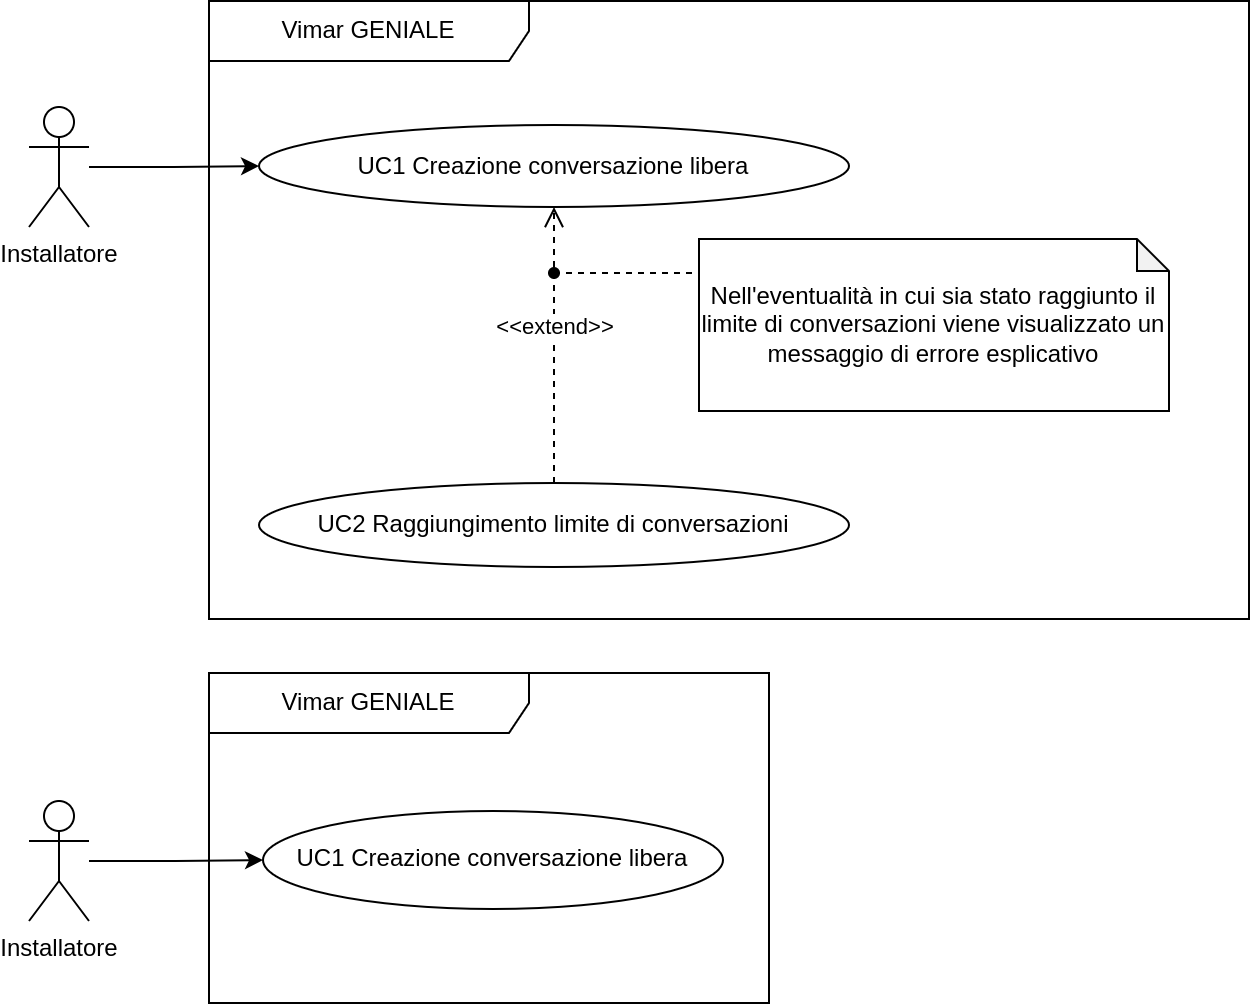
\includegraphics[width=0.8\textwidth]{contents/casi_duso/png/UC1.png}
\caption{UC1 - Creazione conversazione libera}
% \label{fig:UC1a}
\end{figure}

\uc{Raggiungimento limite di conversazioni}{limite_conv}
\begin{itemize}
    \item \textbf{Attori coinvolti}: Installatore;
    \item \textbf{Descrizione}: L’installatore desidera interrogare il sistema, ma quando prova a creare una nuova conversazione per richiedere le informazioni a lui necessarie, supera il limite massimo di conversazioni supportate;
    \item \textbf{Precondizioni}: 
        \begin{itemize}
            \item L’installatore ha accesso all’interfaccia web del sistema;
            \item Il numero di conversazioni memorizzate nel sistema supera il limite massimo supportato;
        \end{itemize}
    \item \textbf{Postcondizioni}:  Il sistema restituisce una risposta che indica il motivo per cui si è verificato l’errore;
    \item \textbf{Scenario principale}:
    \begin{enumerate}
    \item L’installatore accede all’interfaccia web di Vimar GENIALE;
    \item Richiede la creazione di una nuova conversazione, nonostante siano già esistenti un numero di conversazioni che raggiunge il limite;
    \item Il sistema elabora la richiesta e fornisce una risposta che spiega la causa dell'errore riscontrato;
    \item L’installatore visualizza le informazioni sull’errore che si è verificato.
    \end{enumerate}
\end{itemize}
\begin{figure}[H]
\centering
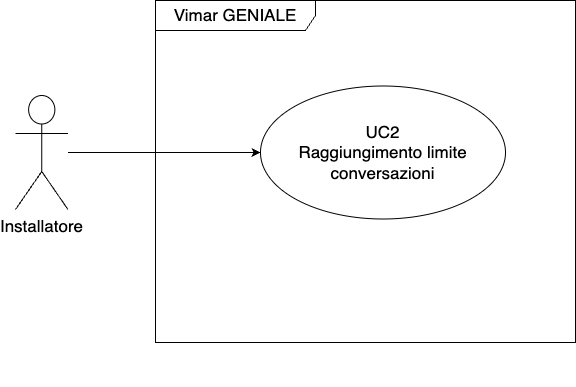
\includegraphics[width=0.8\textwidth]{contents/casi_duso/png/UC2.png}
\caption{UC2 - Raggiungimento limite di conversazioni}
\end{figure}


\uc{Salvataggio conversazione}{salvataggio_conv}
\begin{itemize}
    \item \textbf{Attori coinvolti}: Installatore;
    \item \textbf{Descrizione}: L’installatore, prima di chiudere l’applicativo, desidera salvare le conversazioni memorizzate attualmente all’interno del sistema, per poterle utilizzare nuovamente dal punto in cui ha concluso in precedenza alla prossima apertura dell’applicativo;
    \item \textbf{Precondizioni}: 
        \begin{itemize}
            \item L’installatore ha accesso all’interfaccia web del sistema;
            \item Sono presenti nel sistema un numero consentito di conversazioni;
        \end{itemize}
    \item \textbf{Postcondizioni}: Il sistema salva le conversazioni memorizzate attualmente all’interno del sistema;
    \item \textbf{Scenario principale}:
    \begin{enumerate}
    \item L’installatore accede all’interfaccia web di Vimar GENIALE;
    \item Richiede il salvataggio delle conversazioni esistenti al momento, prima di effettuare la chiusura dell’applicativo;
    \item Il sistema effettua il salvataggio e fornisce una risposta che conferma il completamento dell’operazione;
    \item L’installatore visualizza il messaggio di conferma dell’avvenuto salvataggio.
    \end{enumerate}
    \item \textbf{Estensioni}: UC 4 - Assenza di conversazioni durante il salvataggio
\end{itemize}
\begin{figure}[H]
\centering
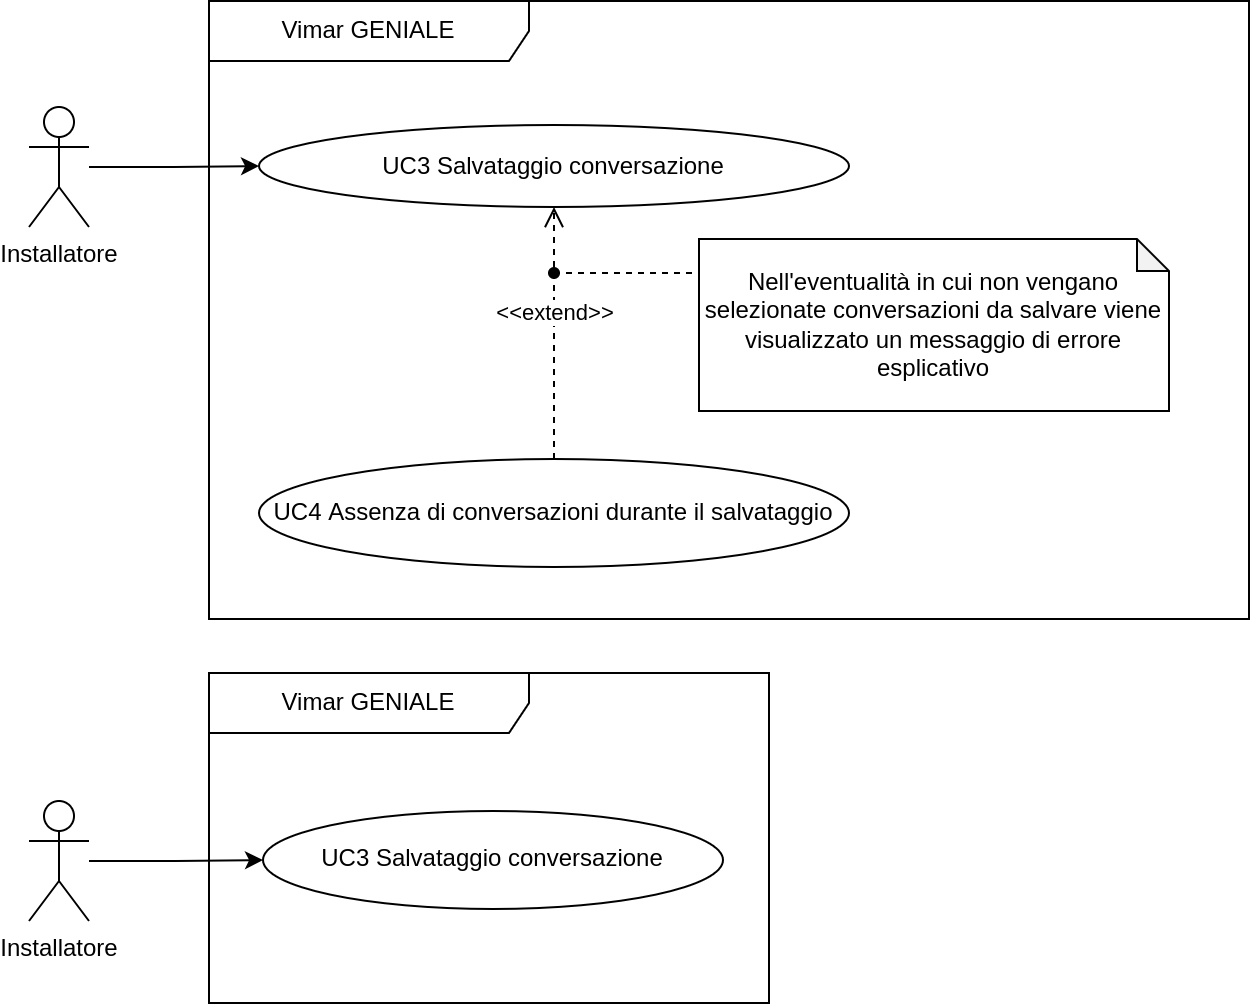
\includegraphics[width=0.8\textwidth]{contents/casi_duso/png/UC3.png}
\caption{UC3 - Salvataggio conversazione}
% \label{fig:UC1a}
\end{figure}

\uc{Assenza di conversazioni durante il salvataggio}{assenza_conv}
\begin{itemize}
    \item \textbf{Attori coinvolti}: Installatore;
    \item \textbf{Descrizione}: L’installatore tenta di salvare una o più conversazioni senza, però, che ce ne sia alcuna;
    \item \textbf{Precondizioni}: 
        \begin{itemize}
            \item L’installatore ha accesso all’interfaccia web del sistema;
            \item L'installatore crea una nuova conversazione libera e poi non fa nessuna domanda.
        \end{itemize}
    \item \textbf{Postcondizioni}: Il sistema restituisce una risposta che indica il motivo per cui si è verificato l’errore;
    \item \textbf{Scenario principale}:
    \begin{enumerate}
    \item L’installatore accede all’interfaccia web di Vimar GENIALE;
    \item L'installatore crea una nuova conversazione, ma non pone nessuna domanda.
    \item Richiede il salvataggio di una o più conversazioni;
    \item Il sistema elabora la richiesta e fornisce una risposta che spiega la causa dell'errore riscontrato;
    \item L’installatore visualizza le informazioni sull’errore che si è verificato.
    \end{enumerate}
\end{itemize}
\begin{figure}[H]
\centering
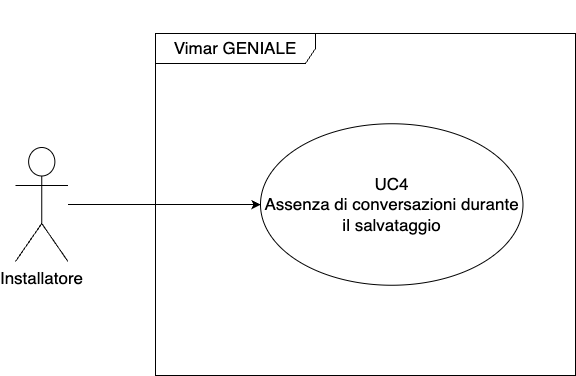
\includegraphics[width=0.8\textwidth]{contents/casi_duso/png/UC4.png}
\caption{UC4 - Assenza di conversazioni durante il salvataggio}
% \label{fig:UC1a}
\end{figure}


\uc{Cancellazione conversazione}{cancellazione_conv}
\begin{itemize}
    \item \textbf{Attori coinvolti}: Installatore;
    \item \textbf{Descrizione}: L’installatore desidera eliminare una conversazione esistente, in quanto non è ritenuta più necessaria al suo scopo;
    \item \textbf{Precondizioni}: 
        \begin{itemize}
            \item L’installatore ha accesso all’interfaccia web del sistema;
            \item L’installatore ha accesso ad una conversazione memorizzata nel sistema;
        \end{itemize}
    \item \textbf{Postcondizioni}: Il sistema elimina la conversazione non ritenuta più necessaria dall’installatore.
    \item \textbf{Scenario principale}:
    \begin{enumerate}
    \item L’installatore accede all’interfaccia web di Vimar GENIALE;
    \item Richiede l’eliminazione di una conversazione, in quanto ha raggiunto il suo scopo e non è più utile;
    \item Il sistema effettua l’eliminazione e fornisce una risposta che conferma il completamento dell’operazione;
    \item L’installatore visualizza il messaggio di conferma dell’avvenuta cancellazione.
    \end{enumerate}
\end{itemize}
\begin{figure}[H]
\centering
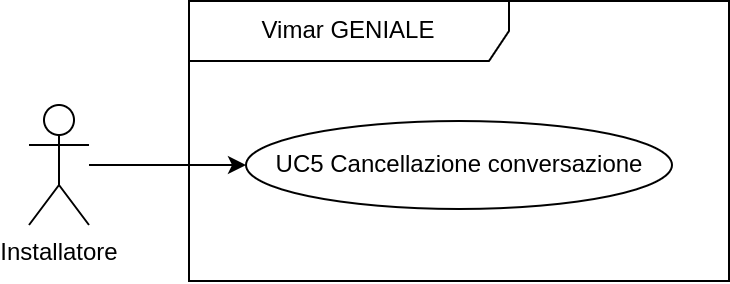
\includegraphics[width=0.8\textwidth]{contents/casi_duso/png/UC5.png}
\caption{UC5 - Cancellazione conversazione}
% \label{fig:UC1a}
\end{figure}


\uc{Ricerca informazioni sui prodotti con conversazione libera}{ricerca_info_prodotti}
\begin{itemize}
    \item \textbf{Attori coinvolti}: Installatore;
    \item \textbf{Descrizione}: L’installatore interroga il sistema per ottenere informazioni dettagliate su un prodotto specifico, come schemi elettrici, dati tecnici e manuali;
    \item \textbf{Precondizioni}: 
        \begin{itemize}
            \item L’installatore ha accesso all’interfaccia web del sistema;
            \item L’installatore ha accesso ad una conversazione memorizzabile nel sistema;
            \item Il prodotto richiesto è registrato nel sistema e le informazioni sono correttamente indicizzate.
        \end{itemize}
    \item \textbf{Postcondizioni}: Il sistema restituisce le informazioni richieste, incluse le descrizioni del prodotto, schemi elettrici e manuali di configurazione;
    \item \textbf{Scenario principale}:
    \begin{enumerate}
    \item L’installatore accede all’interfaccia web di Vimar GENIALE;
    \item Inserisce una domanda o una parola chiave relativa ad un prodotto specifico;
    \item Il sistema esegue la ricerca nel database le informazioni necessarie a fornire sufficiente contesto al LLM.
    \item LLM elabora la risposta;
    \item L’installatore visualizza la risposta.
    \end{enumerate}
    \item \textbf{Estensioni}: 
        \begin{itemize}
            \item UC 7 - Superamento limite caratteri del messaggio
            \item UC 8 - Assenza di informazioni sul prodotto ricercato
        \end{itemize}
\end{itemize}
\begin{figure}[H]
\centering
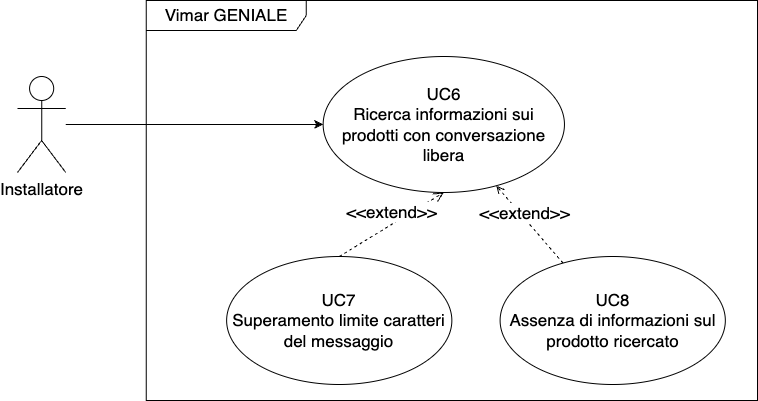
\includegraphics[width=0.8\textwidth]{contents/casi_duso/png/UC6.png}
\caption{UC6 - Ricerca informazioni sui prodotti con conversazione libera}
\end{figure}


\uc{Superamento limite caratteri del messaggio}{superamento_limite_caratteri}
\begin{itemize}
    \item \textbf{Attori coinvolti}: Installatore;
    \item \textbf{Descrizione}: L’installatore, quando interroga il sistema per ottenere informazioni, supera il limite di caratteri che possono essere utilizzati per effettuare la richiesta;
    \item \textbf{Precondizioni}: 
        \begin{itemize}
            \item L’installatore ha accesso all’interfaccia web del sistema;
            \item L’installatore ha accesso ad una conversazione memorizzabile nel sistema;
            \item La domanda posta supera il limite massimo di caratteri consentiti.
        \end{itemize}
    \item \textbf{Postcondizioni}: Il sistema restituisce una risposta che indica il motivo per cui si è verificato l’errore;
    \item \textbf{Scenario principale}:
    \begin{enumerate}
    \item L’installatore accede all’interfaccia web di Vimar GENIALE;
    \item Inserisce una domanda o una parola chiave relativa ad un prodotto specifico, superando il limite massimo consentito di caratteri;
    \item Il sistema elabora la richiesta e fornisce una risposta che spiega la causa dell'errore riscontrato;
    \item L’installatore visualizza le informazioni sull’errore che si è verificato.
    \end{enumerate}
\end{itemize}
\begin{figure}[H]
\centering
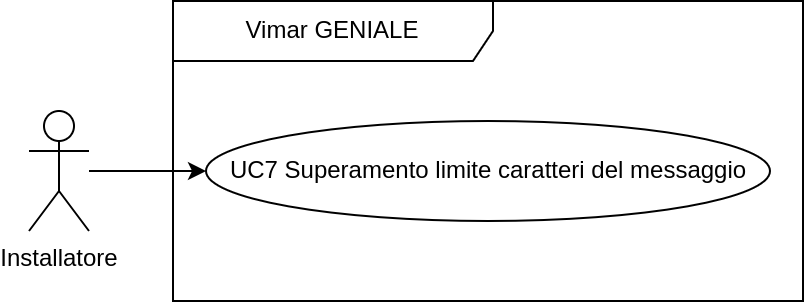
\includegraphics[width=0.8\textwidth]{contents/casi_duso/png/UC7.png}
\caption{UC7 - Superamento limite caratteri del messaggio}
% \label{fig:UC1a}
\end{figure}


\uc{Assenza di informazioni sul prodotto ricercato}{assenza_info_prodotto}
\begin{itemize}
    \item \textbf{Attori coinvolti}: Installatore;
    \item \textbf{Descrizione}: L’installatore interroga il sistema per ottenere informazioni dettagliate su un prodotto specifico, ma il sistema non è in grado di trovare nessuna informazione relativa ad esso;
    \item \textbf{Precondizioni}: 
        \begin{itemize}
            \item L’installatore ha accesso all’interfaccia web del sistema;
            \item L’installatore ha accesso ad una conversazione memorizzabile nel sistema;
            \item L’installatore pone una domanda al sistema;
            \item Il sistema non è in possesso di alcuna informazione relativa al prodotto ricercato.
        \end{itemize}
    \item \textbf{Postcondizioni}: Il sistema restituisce una risposta che indica il motivo per cui si è verificato l’errore;
    \item \textbf{Scenario principale}:
    \begin{enumerate}
    \item L’installatore accede all’interfaccia web di Vimar GENIALE;
    \item Inserisce una domanda o una parola chiave relativa ad un prodotto specifico;
    \item Il sistema elabora la richiesta e fornisce una risposta che spiega la causa dell'errore riscontrato;
    \item L’installatore visualizza le informazioni sull’errore che si è verificato.
    \end{enumerate}
\end{itemize}
\begin{figure}[H]
\centering
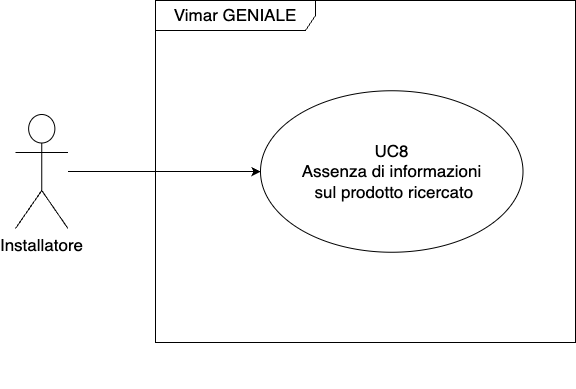
\includegraphics[width=0.8\textwidth]{contents/casi_duso/png/UC8.png}
\caption{UC8 - Assenza di informazioni sul prodotto ricercato}
\end{figure}


\uc{Visualizzazione storico dei messaggi}{visualizzazione_storico_messaggi}
\begin{itemize}
    \item \textbf{Attori coinvolti}: Installatore;
    \item \textbf{Descrizione}: L’installatore, avendo la necessità di riesaminare le risposte ricevute alle domande poste in precedenza, richiede al sistema di mostrare uno storico dei messaggi della conversazione attuale;
    \item \textbf{Precondizioni}: 
        \begin{itemize}
            \item L’installatore ha accesso all’interfaccia web del sistema;
            \item L’installatore ha accesso ad una conversazione memorizzabile nel sistema;
            \item La conversazione attuale contiene dei messaggi che sono stati scambiati in precedenza.
        \end{itemize}
    \item \textbf{Postcondizioni}: Il sistema ritorna lo storico dei messaggi della conversazione attuale.
    \item \textbf{Scenario principale}:
    \begin{enumerate}
    \item L’installatore accede all’interfaccia web di Vimar GENIALE;
    \item Accede ad una conversazione presente nel sistema e richiede di visualizzarne uno storico dei messaggi;
    \item Il sistema elabora la richiesta e fornisce lo storico dei messaggi della conversazione attuale;
    \item L’installatore visualizza i messaggi scambiati in precedenza nella conversazione corrente.
    \end{enumerate}
    \item \textbf{Estensioni}: 
        \begin{itemize}
            \item UC 10 - Mancanza messaggi pregressi nella conversazione
        \end{itemize}
\end{itemize}
\begin{figure}[H]
\centering
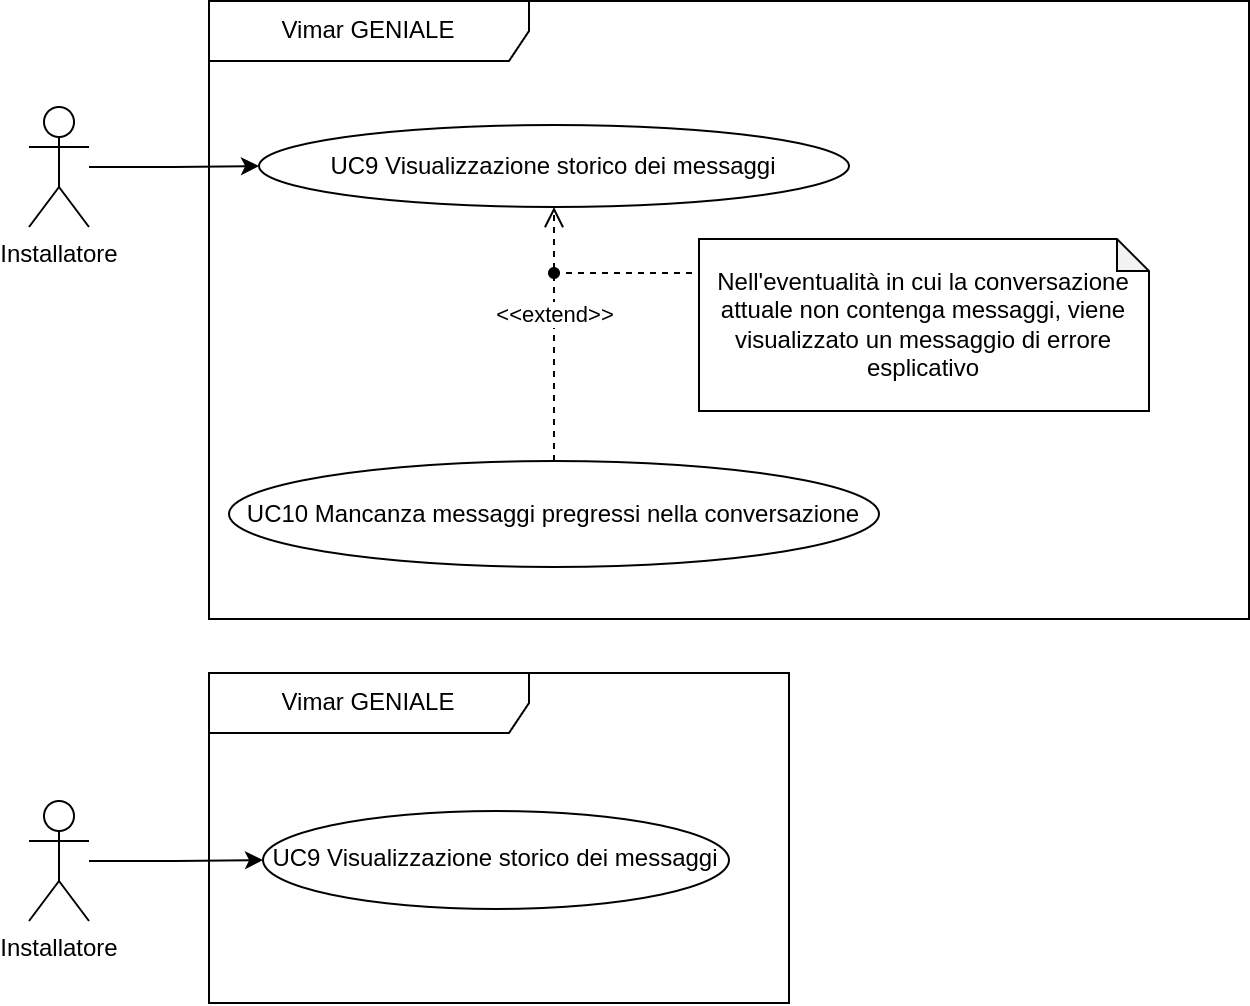
\includegraphics[width=0.8\textwidth]{contents/casi_duso/png/UC9.png}
\caption{UC9 - Visualizzazione storico dei messaggi}
% \label{fig:UC1a}
\end{figure}

\uc{Mancanza messaggi pregressi nella conversazione}{mancanza_messaggi_pregressi}
\begin{itemize}
    \item \textbf{Attori coinvolti}: Installatore;
    \item \textbf{Descrizione}: L’installatore richiede di visualizzare lo storico dei messaggi di una conversazione, ma non ci sono messaggi pregressi nella conversazione attuale;
    \item \textbf{Precondizioni}: 
        \begin{itemize}
            \item L’installatore ha accesso all’interfaccia web del sistema;
            \item L’installatore ha accesso ad una conversazione memorizzabile nel sistema;
            \item La conversazione attuale non contiene messaggi scambiati in precedenza.
        \end{itemize}
    \item \textbf{Postcondizioni}: Il sistema restituisce una risposta che indica l’assenza di messaggi pregressi nella conversazione attuale;
    \item \textbf{Scenario principale}:
    \begin{enumerate}
    \item L’installatore accede all’interfaccia web di Vimar GENIALE;
    \item Accede ad una conversazione presente nel sistema e richiede di visualizzarne uno storico dei messaggi;
    \item Il sistema elabora la richiesta e fornisce una risposta che indica l’assenza di messaggi pregressi nella conversazione attuale;
    \item L’installatore visualizza il messaggio che indica l’assenza di messaggi pregressi.
    \end{enumerate}
\end{itemize}
\begin{figure}[H]
\centering
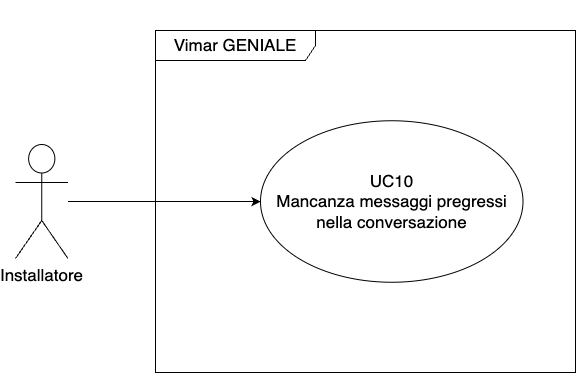
\includegraphics[width=0.8\textwidth]{contents/casi_duso/png/UC10.png}
\caption{UC10 - Mancanza messaggi pregressi nella conversazione}
% \label{fig:UC1a}
\end{figure}


\uc{Fornitura di feedback sulla risposta del sistema ad interrogazione}{fornitura_feedback}
\begin{itemize}
    \item \textbf{Attori coinvolti}: Installatore;
    \item \textbf{Descrizione}: L’installatore, a seguito dell’interrogazione del sistema per ottenere informazioni, desidera fornire un feedback che indichi se la risposta ricevuta sia corretta o meno;
    \item \textbf{Precondizioni}: 
        \begin{itemize}
            \item L’installatore ha accesso all’interfaccia web del sistema;
            \item L’installatore ha accesso ad una conversazione memorizzabile nel sistema;
            \item Il sistema fornisce una risposta ad un’interrogazione da parte dell’installatore.
        \end{itemize}
    \item \textbf{Postcondizioni}: L’installatore, dopo aver esaminato la risposta ricevuta, fornisce un riscontro sulla correttezza di quest’ultima che verrà registrato dal sistema;
    \item \textbf{Scenario principale}:
    \begin{enumerate}
    \item L’installatore accede all’interfaccia web di Vimar GENIALE;
    \item Inserisce una domanda o una parola chiave relativa ad un prodotto specifico;
    \item Il sistema esegue la ricerca nel database dei prodotti e restituisce una risposta che include informazioni dettagliate come schemi, descrizioni e manuali;
    \item L’installatore visualizza le informazioni fornite e, dopo aver verificato la correttezza delle informazioni ricevute, fornisce un feedback sulla risposta al sistema;
    \item Il sistema registra il feedback ricevuto dall’installatore.
    \end{enumerate}
    \item \textbf{Inclusioni} (Le inclusioni hanno senso se verranno svolte azioni aggiuntive rispetto alla sola registrazione del feedback): 
        \begin{itemize}
            \item UC 11.1 - Fornitura di feedback positivo sulla risposta del sistema ad interrogazione
            \item UC 11.2 - Fornitura di feedback negativo sulla risposta del sistema ad interrogazione
        \end{itemize}
\end{itemize}

\subuc{Fornitura di feedback positivo sulla risposta del sistema ad interrogazione}{feedback_positivo}
\begin{itemize}
    \item \textbf{Attori coinvolti}: Installatore;
    \item \textbf{Descrizione}: L’installatore, a seguito dell’interrogazione del sistema per ottenere informazioni, desidera fornire un feedback che indichi che la risposta ricevuta è corretta;
    \item \textbf{Precondizioni}: 
        \begin{itemize}
            \item L’installatore ha accesso all’interfaccia web del sistema;
            \item L’installatore ha accesso ad una conversazione memorizzata nel sistema;
            \item Il sistema fornisce una risposta corretta ad un’interrogazione da parte dell’installatore.
        \end{itemize}
    \item \textbf{Postcondizioni}: L’installatore, dopo aver esaminato la risposta ricevuta, fornisce un riscontro positivo sulla correttezza di quest’ultima che verrà registrato dal sistema;
    \item \textbf{Scenario principale}:
    \begin{enumerate}
    \item L’installatore accede all’interfaccia web di Vimar GENIALE;
    \item Inserisce una domanda o una parola chiave relativa ad un prodotto specifico;
    \item Il sistema esegue la ricerca nel database dei prodotti e restituisce una risposta che include informazioni dettagliate come schemi, descrizioni e manuali;
    \item L’installatore visualizza le informazioni fornite e, dopo aver verificato la correttezza delle informazioni ricevute, fornisce un feedback positivo sulla risposta al sistema;
    \item Il sistema registra il feedback ricevuto dall’installatore.
    \end{enumerate}
\end{itemize}

\subuc{Fornitura di feedback negativo sulla risposta del sistema ad interrogazione}{feedback_negativo}
\begin{itemize}
    \item \textbf{Attori coinvolti}: Installatore;
    \item \textbf{Descrizione}: L’installatore, a seguito dell’interrogazione del sistema per ottenere informazioni, desidera fornire un feedback che indichi che la risposta ricevuta è errata;
    \item \textbf{Precondizioni}: 
        \begin{itemize}
            \item L’installatore ha accesso all’interfaccia web del sistema;
            \item L’installatore ha accesso ad una conversazione memorizzata nel sistema;
            \item Il sistema fornisce una risposta errata ad un’interrogazione da parte dell’installatore.
        \end{itemize}
    \item \textbf{Postcondizioni}: L’installatore, dopo aver esaminato la risposta ricevuta, fornisce un riscontro negativo sulla correttezza di quest’ultima che verrà registrato dal sistema;
    \item \textbf{Scenario principale}:
    \begin{enumerate}
    \item L’installatore accede all’interfaccia web di Vimar GENIALE;
    \item Inserisce una domanda o una parola chiave relativa ad un prodotto specifico;
    \item Il sistema esegue la ricerca nel database dei prodotti e restituisce una risposta che include informazioni dettagliate come schemi, descrizioni e manuali;
    \item L’installatore visualizza le informazioni fornite e, dopo aver verificato la correttezza delle informazioni ricevute, fornisce un feedback negativo sulla risposta al sistema;
    \item Il sistema registra il feedback ricevuto dall’installatore.
    \end{enumerate}
\end{itemize}
\begin{figure}[H]
\centering
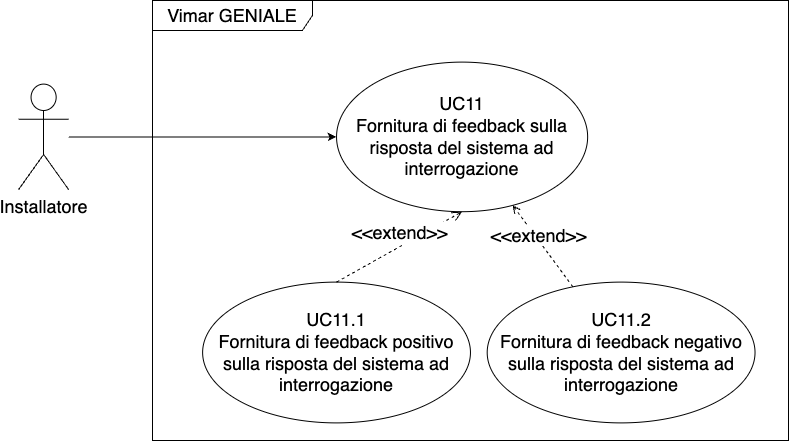
\includegraphics[width=0.8\textwidth]{contents/casi_duso/png/UC11.png}
\caption{UC11 - Fornitura di feedback sulla risposta del sistema ad interrogazione}
% \label{fig:UC1a}
\end{figure}

\uc{Accesso al cruscotto informativo}{accesso_cruscotto}
\begin{itemize}
    \item \textbf{Attori coinvolti}: Amministratore;
    \item \textbf{Descrizione}: Un amministratore desidera accedere al cruscotto informativo per visualizzare una panoramica di informazioni relative all’utilizzo del sistema;
    \item \textbf{Precondizioni}: 
        \begin{itemize}
            \item L’amministratore ha accesso all’interfaccia web del sistema;
            \item L’amministratore è dotato delle credenziali necessarie ad accedere alla dashboard.
        \end{itemize}
    \item \textbf{Postcondizioni}: L’amministratore accede al cruscotto informativo, da cui può visualizzare svariate informazioni riguardanti l’uso del sistema;
    \item \textbf{Scenario principale}:
    \begin{enumerate}
    \item L’amministratore accede all’interfaccia web di Vimar GENIALE;
    \item Inserisce le proprie credenziali;
    \item Il sistema riceve la richiesta di accesso e verifica le credenziali;
    \item L’amministratore ottiene l’accesso alla dashboard.
    \end{enumerate}
    \item \textbf{Estensioni}: UC 13 - Inserimento username o password errati
    \item \textbf{Inclusioni}: 
        \begin{itemize}
            \item UC 12.1 - Inserimento username e password
        \end{itemize}
\end{itemize}


\subuc{Inserimento username e password}{inserimento_username}
\begin{itemize}
    \item \textbf{Attori coinvolti}: Amministratore;
    \item \textbf{Descrizione}: Un amministratore desidera accedere al cruscotto informativo per visualizzare una panoramica di informazioni relative all’utilizzo del sistema, dunque inserisce lo username e la password;
    \item \textbf{Precondizioni}: 
        \begin{itemize}
            \item L’amministratore ha accesso all’interfaccia web del sistema;
            \item L’amministratore è dotato dello username e della password necessarie ad accedere alla dashboard.
        \end{itemize}
    \item \textbf{Postcondizioni}: L’amministratore ha inserito lo username e la password, ovvero le credenziali richieste per l’accesso al cruscotto informativo;
    \item \textbf{Scenario principale}:
    \begin{enumerate}
    \item L’amministratore accede all’interfaccia web di Vimar GENIALE;
    \item Inserisce lo username.
    \item Inserisce la password.
    \end{enumerate}
\end{itemize}


\uc{Inserimento username o password errati}{inserimento_cred_errati}
\begin{itemize}
    \item \textbf{Attori coinvolti}: Amministratore;
    \item \textbf{Descrizione}: Un amministratore desidera accedere al cruscotto informativo per visualizzare una panoramica di informazioni relative all’utilizzo del sistema, ma non riesce ad accedere a causa di un errore nell’inserimento dello username o della password;
    \item \textbf{Precondizioni}: 
        \begin{itemize}
            \item L’amministratore ha accesso all’interfaccia web del sistema;
            \item L’amministratore è dotato delle credenziali necessarie ad accedere alla dashboard;
            \item Lo username o la password non sono corretti.
        \end{itemize}
    \item \textbf{Postcondizioni}: Il sistema restituisce una risposta che indica il motivo per cui si è verificato l’errore;
    \item \textbf{Scenario principale}:
    \begin{enumerate}
    \item L’amministratore accede all’interfaccia web di Vimar GENIALE;
    \item Inserisce le proprie credenziali;
    \item Il sistema elabora la richiesta e fornisce una risposta che spiega l’inserimento errato delle credenziali;
    \item L’amministratore visualizza le informazioni sull’errore che si è verificato.
    \end{enumerate}
\end{itemize}

\begin{figure}[H]
\centering
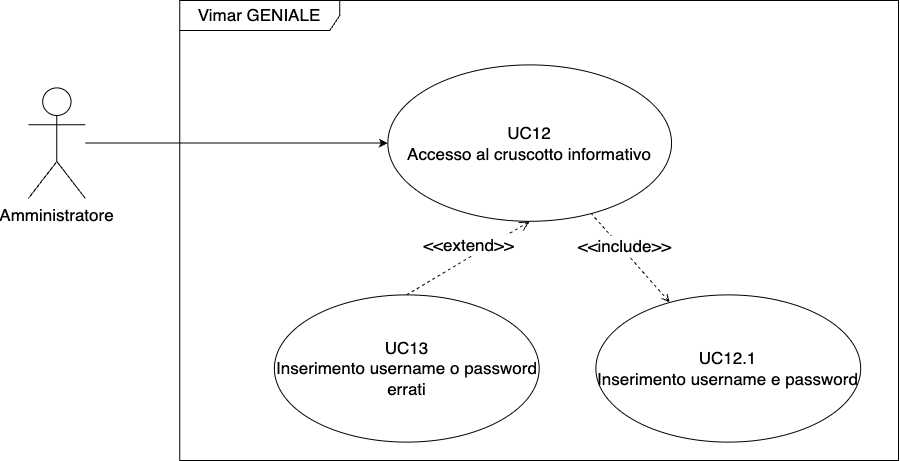
\includegraphics[width=0.8\textwidth]{contents/casi_duso/png/UC12.png}
\caption{UC12, UC12.1 UC13 - Accesso al cruscotto informativo }
% \label{fig:UC1a}
\end{figure}

\uc{Visualizzazione informazioni sulla dashboard}{visualizzazione_info_dashboard}
\begin{itemize}
    \item \textbf{Attori coinvolti}: Amministratore;
    \item \textbf{Descrizione}: Un amministratore desidera visualizzare una panoramica di informazioni relative all’utilizzo del sistema dal cruscotto informativo;
    \item \textbf{Precondizioni}: 
        \begin{itemize}
            \item L’amministratore ha accesso all’interfaccia web del sistema;
            \item L’amministratore è dotato dell’accesso alla dashboard;
        \end{itemize}
    \item \textbf{Postcondizioni}: Il sistema raccoglie le informazioni richieste e le mostra nella dashboard;
    \item \textbf{Scenario principale}:
    \begin{enumerate}
    \item L’amministratore accede all’interfaccia web di Vimar GENIALE;
    \item Inserisce le proprie credenziali;
    \item Il sistema riceve la richiesta di accesso e verifica le credenziali;
    \item L’amministratore ottiene l’accesso alla dashboard;
    \item Il sistema mostra le informazioni richieste sul cruscotto informativo.
    \end{enumerate}
    \item \textbf{Inclusioni}: UC 12 - Accesso al cruscotto informativo
\end{itemize}

\subuc{Visualizzazione numero richieste con conversazione libera}{visualizzazione_richieste_libere}
\begin{itemize}
    \item \textbf{Attori coinvolti}: Amministratore;
    \item \textbf{Descrizione}: Un amministratore desidera visualizzare dal cruscotto informativo il numero delle richieste effettuate con una conversazione libera;
    \item \textbf{Precondizioni}: 
        \begin{itemize}
            \item L’amministratore ha accesso all’interfaccia web del sistema;
            \item L’amministratore è dotato dell’accesso alla dashboard;
        \end{itemize}
    \item \textbf{Postcondizioni}: Il sistema raccoglie le informazioni relative al numero delle richieste effettuate con una conversazione libera e le mostra nella dashboard;
    \item \textbf{Scenario principale}:
    \begin{enumerate}
    \item L’amministratore accede all’interfaccia web di Vimar GENIALE;
    \item Inserisce le proprie credenziali;
    \item Il sistema riceve la richiesta di accesso e verifica le credenziali;
    \item L’amministratore ottiene l’accesso alla dashboard;
    \item Il sistema mostra le informazioni richieste sul cruscotto informativo.
    \end{enumerate}
    \item \textbf{Inclusioni}: UC 12 - Accesso al cruscotto informativo
    \item \textbf{Generalizzazioni}: UC 14 - Visualizzazione informazioni sulla dashboard
\end{itemize}

\subuc{Visualizzazione numero richieste con conversazione guidata}{visualizzazione_richieste_guidate}
\begin{itemize}
    \item \textbf{Attori coinvolti}: Amministratore;
    \item \textbf{Descrizione}: Un amministratore desidera visualizzare dal cruscotto informativo il numero delle richieste effettuate con una conversazione guidata;
    \item \textbf{Precondizioni}: 
        \begin{itemize}
            \item L’amministratore ha accesso all’interfaccia web del sistema;
            \item L’amministratore è dotato dell’accesso alla dashboard;
        \end{itemize}
    \item \textbf{Postcondizioni}: Il sistema raccoglie le informazioni relative al numero delle richieste effettuate con una conversazione guidata e le mostra nella dashboard;
    \item \textbf{Scenario principale}:
    \begin{enumerate}
    \item L’amministratore accede all’interfaccia web di Vimar GENIALE;
    \item Inserisce le proprie credenziali;
    \item Il sistema riceve la richiesta di accesso e verifica le credenziali;
    \item L’amministratore ottiene l’accesso alla dashboard;
    \item Il sistema mostra le informazioni richieste sul cruscotto informativo.
    \end{enumerate}
    \item \textbf{Inclusioni}: UC 12 - Accesso al cruscotto informativo
    \item \textbf{Generalizzazioni}: UC 14 - Visualizzazione informazioni sulla dashboard
\end{itemize}

\subuc{Visualizzazione statistiche sul numero di parole usate nelle richieste}{visualizzazione_statistiche_parole}
\begin{itemize}
    \item \textbf{Attori coinvolti}: Amministratore;
    \item \textbf{Descrizione}: Un amministratore desidera visualizzare dal cruscotto informativo le statistiche sul numero di parole utilizzate;
    \item \textbf{Precondizioni}: 
        \begin{itemize}
            \item L’amministratore ha accesso all’interfaccia web del sistema;
            \item L’amministratore è dotato dell’accesso alla dashboard;
        \end{itemize}
    \item \textbf{Postcondizioni}: Il sistema raccoglie le informazioni relative alle statistiche sul numero di termini utilizzati nelle richieste e le mostra nella dashboard;
    \item \textbf{Scenario principale}:
    \begin{enumerate}
    \item L’amministratore accede all’interfaccia web di Vimar GENIALE;
    \item Inserisce le proprie credenziali;
    \item Il sistema riceve la richiesta di accesso e verifica le credenziali;
    \item L’amministratore ottiene l’accesso alla dashboard;
    \item Il sistema mostra le informazioni richieste sul cruscotto informativo.
    \end{enumerate}
    \item \textbf{Inclusioni}: UC 12 - Accesso al cruscotto informativo
    \item \textbf{Generalizzazioni}: UC 14 - Visualizzazione informazioni sulla dashboard
\end{itemize}

\subuc{Visualizzazione numero risposte positive dal sistema di feedback}{visualizzazione_risposte_positive}
\begin{itemize}
    \item \textbf{Attori coinvolti}: Amministratore;
    \item \textbf{Descrizione}: Un amministratore desidera visualizzare dal cruscotto informativo il numero delle risposte positive dal sistema di feedback;
    \item \textbf{Precondizioni}: 
        \begin{itemize}
            \item L’amministratore ha accesso all’interfaccia web del sistema;
            \item L’amministratore è dotato dell’accesso alla dashboard;
        \end{itemize}
    \item \textbf{Postcondizioni}: Il sistema raccoglie le informazioni relative al numero delle risposte positive dal sistema di feedback e le mostra nella dashboard;
    \item \textbf{Scenario principale}:
    \begin{enumerate}
    \item L’amministratore accede all’interfaccia web di Vimar GENIALE;
    \item Inserisce le proprie credenziali;
    \item Il sistema riceve la richiesta di accesso e verifica le credenziali;
    \item L’amministratore ottiene l’accesso alla dashboard;
    \item Il sistema mostra le informazioni richieste sul cruscotto informativo.
    \end{enumerate}
    \item \textbf{Inclusioni}: UC 12 - Accesso al cruscotto informativo
    \item \textbf{Generalizzazioni}: UC 14 - Visualizzazione informazioni sulla dashboard
\end{itemize}

\subuc{Visualizzazione numero risposte negative dal sistema di feedback}{visualizzazione_risposte_negative}
\begin{itemize}
    \item \textbf{Attori coinvolti}: Amministratore;
    \item \textbf{Descrizione}: Un amministratore desidera visualizzare dal cruscotto informativo il numero delle risposte negative dal sistema di feedback;
    \item \textbf{Precondizioni}: 
        \begin{itemize}
            \item L’amministratore ha accesso all’interfaccia web del sistema;
            \item L’amministratore è dotato dell’accesso alla dashboard;
        \end{itemize}
    \item \textbf{Postcondizioni}: Il sistema raccoglie le informazioni relative al numero delle risposte negative dal sistema di feedback e le mostra nella dashboard;
    \item \textbf{Scenario principale}:
    \begin{enumerate}
    \item L’amministratore accede all’interfaccia web di Vimar GENIALE;
    \item Inserisce le proprie credenziali;
    \item Il sistema riceve la richiesta di accesso e verifica le credenziali;
    \item L’amministratore ottiene l’accesso alla dashboard;
    \item Il sistema mostra le informazioni richieste sul cruscotto informativo.
    \end{enumerate}
    \item \textbf{Inclusioni}: UC 12 - Accesso al cruscotto informativo
    \item \textbf{Generalizzazioni}: UC 14 - Visualizzazione informazioni sulla dashboard
\end{itemize}
\begin{figure}[H]
\centering
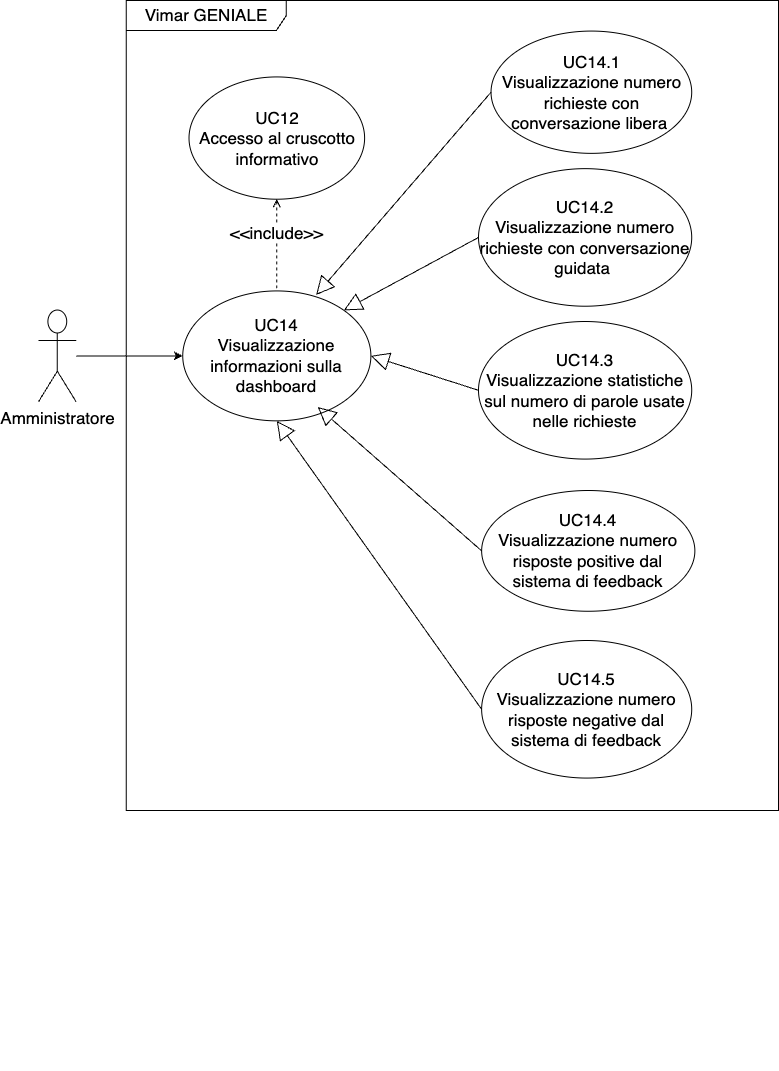
\includegraphics[width=0.8\textwidth]{contents/casi_duso/png/UC14.png}
\caption{UC14 - Visualizzazione informazioni dashboard}
% \label{fig:UC1a}
\end{figure}


\uc{Richiesta di argomento proibito}{argomento_proibito}
\begin{itemize}
    \item \textbf{Attori coinvolti}: Installatore;
    \item \textbf{Descrizione}: L’installatore richiede argomenti proibiti al sistema (e.g. politica, finanza, pornografia, ...);
    \item \textbf{Precondizioni}: 
        \begin{itemize}
            \item L’installatore ha accesso all’interfaccia web del sistema;
            \item L’installatore ha accesso ad una conversazione memorizzabile nel sistema;
            \item La domanda posta non riguarda argomenti proibiti.
        \end{itemize}
    \item \textbf{Postcondizioni}: Il sistema restituisce una risposta che indica il motivo per cui si è verificato l’errore;
    \item \textbf{Scenario principale}:
    \begin{enumerate}
    \item L’installatore accede all’interfaccia web di Vimar GENIALE;
    \item Inserisce una domanda inconsistente, che non ha a che vedere con prodotti VIMAR;
    \item Il sistema elabora la richiesta e fornisce una risposta che spiega la causa dell'errore riscontrato;
    \item L’installatore visualizza le informazioni sull’errore che si è verificato;
    \end{enumerate}
     \item \textbf{Generalizzazioni}: UC 8 - Assenza di informazioni sul prodotto ricercato.
\end{itemize}
\begin{figure}[H]
\centering
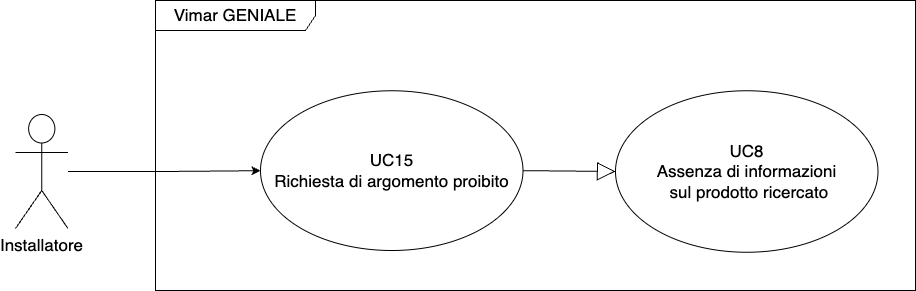
\includegraphics[width=0.8\textwidth]{contents/casi_duso/png/UC15.png}
\caption{UC15 - Richiesta di argomento proibito}
% \label{fig:UC1a}
\end{figure}

\uc{Domanda al sisitema}{domanda}
\begin{itemize}
    \item \textbf{Attori coinvolti}: Installatore;
    \item \textbf{Descrizione}: L’installatore inserisce una domanda;
    \item \textbf{Precondizioni}: 
        \begin{itemize}
            \item L’installatore ha accesso all’interfaccia web del sistema;
            \item L’installatore ha accesso ad una conversazione memorizzabile nel sistema;
            \item L'installatore ha inviato una domanda al sistema;
            \item La domanda posta non riguarda argomenti proibiti.
        \end{itemize}
    \item \textbf{Postcondizioni}: Il sistema restituisce una risposta;
    \item \textbf{Scenario principale}:
    \begin{enumerate}
    \item L’installatore accede all’interfaccia web di Vimar GENIALE;
    \item Inserisce una domanda che ha a che vedere con prodotti VIMAR e non con argomenti proibiti o sconosciuti;
    \item Il sistema elabora la richiesta e fornisce una risposta;
    \item L’installatore visualizza le informazioni restituite;
    \end{enumerate}
    \item \textbf{Estensioni}: UC 17 - Richiesta di uno schema o immagine.
\end{itemize}
\begin{figure}[H]
\centering
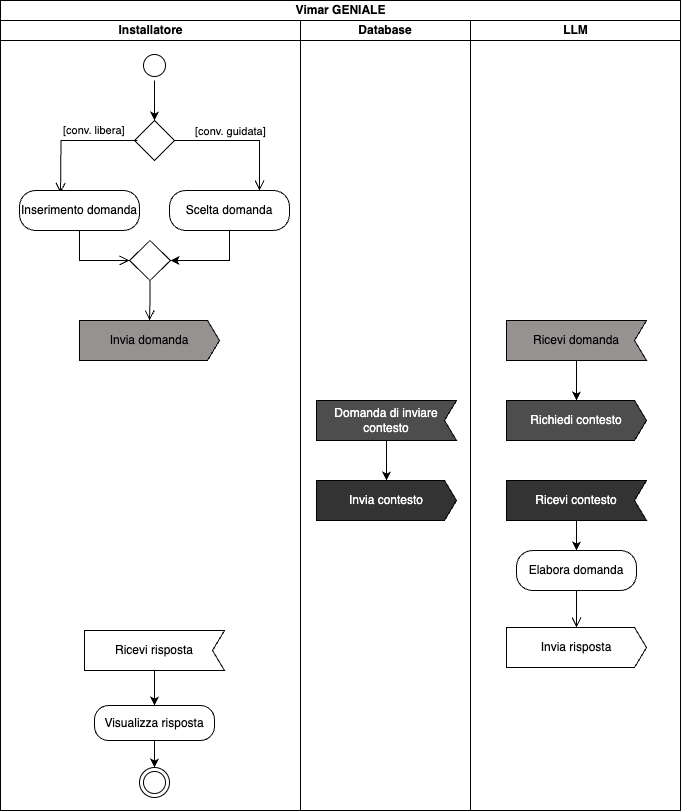
\includegraphics[width=0.8\textwidth]{contents/casi_duso/png/UC16_activity.png}
\caption{UC16 - Domanda al sisitema}
% \label{fig:UC1a}
\end{figure}

\uc{Richiesta di uno schema o immagine}{domanda_immagine}
\begin{itemize}
    \item \textbf{Attori coinvolti}: Installatore;
    \item \textbf{Descrizione}: L’installatore inserisce una domanda la cui risposta prevede uno schema elettrico o un'immagine;
    \item \textbf{Precondizioni}: 
        \begin{itemize}
            \item L’installatore ha accesso all’interfaccia web del sistema;
            \item L’installatore ha accesso ad una conversazione memorizzabile nel sistema;
            \item L'installatore ha inviato una domanda al sistema;
            \item La risposta alla domanda posta necessita, per essere completa, si uno schema elettrico o di un'immagine.
        \end{itemize}
    \item \textbf{Postcondizioni}: Il sistema restituisce una risposta con l'immagine o lo schema corretto;
    \item \textbf{Scenario principale}:
    \begin{enumerate}
    \item L’installatore accede all’interfaccia web di Vimar GENIALE;
    \item Inserisce una domanda che ha a che vedere con prodotti VIMAR;
    \item Il sistema elabora la richiesta e fornisce una risposta inserendo uno schema o di un'immagine di cui la risposta ha bisogno per essere esaustiva;
    \item L’installatore visualizza le informazioni restituite;
    \item \textbf{Inclusioni}: UC 16 - Domanda al sistema.
    \end{enumerate}
\end{itemize}
\begin{figure}[H]
\centering
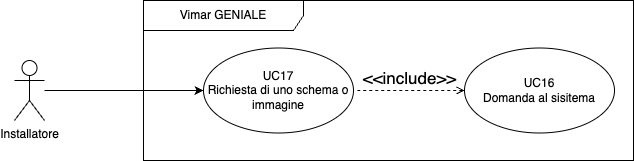
\includegraphics[width=0.8\textwidth]{contents/casi_duso/png/UC17.png}
\caption{UC17 - Richiesta di uno schema o immagine}
% \label{fig:UC1a}
\end{figure}
\newpage
\section{Requisiti}
In questa sezione verranno elencati tutti i requisiti specificati nel capitolato, organizzandoli in categorie distinte per una maggiore chiarezza. Ogni requisito è identificato in modo univoco da un codice, strutturato secondo un formato predefinito, che ne facilita la consultazione e il riferimento all'interno della documentazione con il seguente formato: 
\begin{center}
\textbf{R[Tipo].[Importanza].[Codice]}
\end{center}
dove:
\begin{itemize}
    \item \textbf{Numero:} un numero progressivo a tre cifre che parte dal numero 001.
    \item \textbf{Tipo:} la tipologia di requisito che può essere tra le seguenti:
    \begin{itemize}[label=-]
        \item \textbf{F (funzionale):} Una funzione di sistema descrive il modo in cui un sistema utilizza determinati ingressi per generare specifiche uscite, seguendo una logica o una regola prestabilita che definisce il suo comportamento.
        \item \textbf{Q (qualità):} definisce le caratteristiche di qualità del prodotto software.
        \item \textbf{V (vincolo):} specifica i limiti e le restrizioni imposte dal capitolato, che il prodotto software deve rispettare.
\end{itemize}
    \item \textbf{Priorità:} la priorità viene assegnata al requisito con:
    \begin{itemize}
     \item \textbf{O}: requisito obbligatorio che deve essere soddisfatto per la realizzazione del prodotto software;
        \item \textbf{D}: requisito desiderabile il cui soddisfacimento è apprezzato dal committente;
        \item \textbf{P}: requisito facoltativo, la cui realizzazione è totalmente a discrezione del team in base all'andamento del progetto.
    \end{itemize}
\end{itemize}
In alcuni casi sarà specificato nella colonna delle fonti se il requisito è stato esplicitamente indicato nel Capitolato oppure se è stato dedotto implicitamente da altri requisiti obbligatori. In quest’ultimo caso, si farà riferimento a un requisito interno.
\subsection{Registro di Funzionalità}
\begin{table}[H]
    \begin{tabular}{|C{2.7cm}|L{7.2cm}|C{2.7cm}|C{2cm}|}
        \hline
        \textbf{ID requisito} & \textbf{Descrizione} & \textbf{Importanza} & \textbf{Fonti}  \\
        \hline
        RF.O.1 & Il sistema deve permettere all'installatore di effettuare ricerche testuali e ricevere informazioni dettagliate sui prodotti Vimar. & Obbligatorio & Capitolato \\
        \hline
        RF.O.2 & Il sistema deve prevedere un sistema di autenticazione tramite password per l'accesso alla dashboard per amministratori. & Obbligatorio & UC12 \\
        \hline
        RF.O.3 & Il cruscotto informativo deve includere una sezione per la visualizzazione di statistiche di utilizzo. & Obbligatorio & UC14 \\
        \hline
        RF.O.4 & Il sistema deve permettere agli utenti di fornire un feedback positivo o negativo dopo ogni risposta ricevuta. & Obbligatorio & UC14 \\
        \hline
        RF.O.5 & Il sistema deve essere in grado di identificare e bloccare le richieste che riguardano argomenti non pertinenti ai prodotti VIMAR. & Obbligatorio & UC15 \\
        \hline
        RF.D.6 & Il sistema potrebbe includere la possibilità di visualizzare link di riferimento alle fonti delle informazioni fornite. & Desiderabile & Capitolato \\
        \hline
        RF.P.7 & Il sistema deve fornire un'interfaccia con menu e sottomenù per costruire richieste specifiche in conversazioni guidate & Opzionale & Capitolato\\
        \hline
        RF.O.8 & Il sistema deve consentire solo conversazioni pertinendi ai prodotti Vimar e bloccare conversazioni su argomenti proibiti & Obbligatorio & Capitolato \\
        \hline
        \end{tabular}

\end{table}
\subsection{Registro di Qualità}
\begin{table}[H]
    \begin{tabular}{|C{2.7cm}|L{7.2cm}|C{2.7cm}|C{2cm}|}
        \hline
        \textbf{ID requisito} & \textbf{Descrizione} & \textbf{Importanza} & \textbf{Fonti}  \\
        \hline
       
        \hline
        RQ.O.1 & L'interfaccia utente del sistema potrebbe essere responsive, adattandosi a diversi dispositivi. & Desiderabile & Capitolato \\
        \hline
        RQ.O.2 & Il sistema deve essere progettato per essere facilmente eseguibile su altri dispositivi tramite tecnologia container. & Obbligatorio & Capitolato \\
        \hline
        
        \end{tabular}

\end{table}
\subsection{Requisiti di Vincolo}
\begin{table}[H]
     \begin{tabular}{|C{2.7cm}|L{7.2cm}|C{2.7cm}|C{2cm}|}
        \hline
    \textbf{ID requisito} & \textbf{Descrizione} & \textbf{Importanza} & \textbf{Fonti}  \\
    \hline
           RV.O.1 & Il sistema deve integrare un modello AI (LLM) open source. & Obbligatorio & Capitolato \\
          \hline 
          RV.O.2 & L'infrastruttura deve utilizzare Docker e rispettare il principio di Infrastructure as Code & Obbligatorio & Capitolato \\
          RV.D.3 & L'applicativo può essere ospitato su AWS & Desiderabile & Capitolato \\
          \hline
    \end{tabular}

\end{table}
\newpage
\section{Tracciamento Requisiti}
\begin{table}[H]
\centering
    \begin{tabular}{|C{3.0cm}|C{3.0cm}|}
        \hline
         \textbf{Fonte} &
         \textbf{ID requisito}   
          \\
          \hline
          Capitolato & R-XXX-X-X \\
          \hline 
          Interno & R-XXX-X-X \\
          \hline
    \end{tabular}
     \caption{Requisiti}
\end{table}
\subsection{Riepilogo}
\begin{table}[H]
\centering
    \begin{tabular}{|C{3.0cm}|C{2.5cm}|C{2.5cm}|C{2.5cm}|}
        \hline
         \textbf{Tipologia} &
         \textbf{Obbligatori} & 
         \textbf{Desiderabili} &
         \textbf{Funzionali} 
          \\
          \hline
          \textbf{Funzionali} & 00 & 00 & 00 \\
          \hline 
          \textbf{Qualità} & 00 & 00 & 00\\
          \hline
          \textbf{Vincolo} & 00 & 00 & 00\\
          \hline
    \end{tabular}
    \caption{Requisiti per tipologia}
\end{table}
\subsection{Conclusioni}
\newpage
\end{document}
